%% Mapping (chpt5)
The task of mapping was the main challenge of this work. This task consists in placing recognizable features in a map, that can later be used as landmarks by the drone to estimate its own position. The main challenge in the 3D case, is that a point needs to be observed from at least 2 different positions to be mapped. The simplest approach to map a point, is to simply triangulate its position from two different views. We will begin by exploring this approach. We will find that although this does work reasonably well when we are certain of the position of the cameras, it does not when this position is uncertain. In addition, this method does not allow to take more than two views into account. To remedy these problems we will implement a bundle adjustment step, that allows to build a map that is globally consistent. Throughout this section, we will have to make design choices to try to obtain a method that is both fast enough to work in real time, and accurate enough for the drone to control its position. To evaluate these performances, we will perform a standardized test.

\section{Evaluation procedure} \label{evalproc}
The evaluation will happen in two phases: first the drone will initialize its map and then it will be moved to various known locations, and we will measure the accuracy of its position estimation. The setup used for this evaluation is illustrated on figure \ref{fig:benchmarksetup}. During the initialization phase, we will try to emulate the way the drone would initialize its map just after taking off during a real flight mission (see more in section %TODO
). First the drone is place in a know position on a table (position A in figure \ref{fig:benchmarksetup}). There, the drone is turned on, and it begins initializing its map. The drone is then successively places in 3 other known locations (B, then C, then D), and at each of these locations, the drone in manually communicated its position. Every time this happens, the drone adds landmarks into the map, and optionally updates existing landmarks' position, or even removes some landmarks. In reality, the drone would not know its exact position when taking views at points B, C, and D (position A is defined as the origin), especially at the beginning, as it would have to rely on its IMU and other internal sensors to estimate its position. To emulate this, we implement a second type of test: the robustness test, where the position that is communicated to the drone is slightly different from its real position, at each of the uncertain points (B, C, and D).\\
In the second phase of the evaluation, the drone is again placed at different known locations. This time, no information is communicated to the drone from the outside, and the drone does not modify its map. The drone estimates its position using only its camera and the map that it built during the initialization phase. We compare the drone's estimated position with its real position to evaluate the quality of the map. The two quantities we will seek to optimize are the accuracy of the drone's postition estimation, and the time taken to compute the map.


\begin{figure}[H]
  \centering
  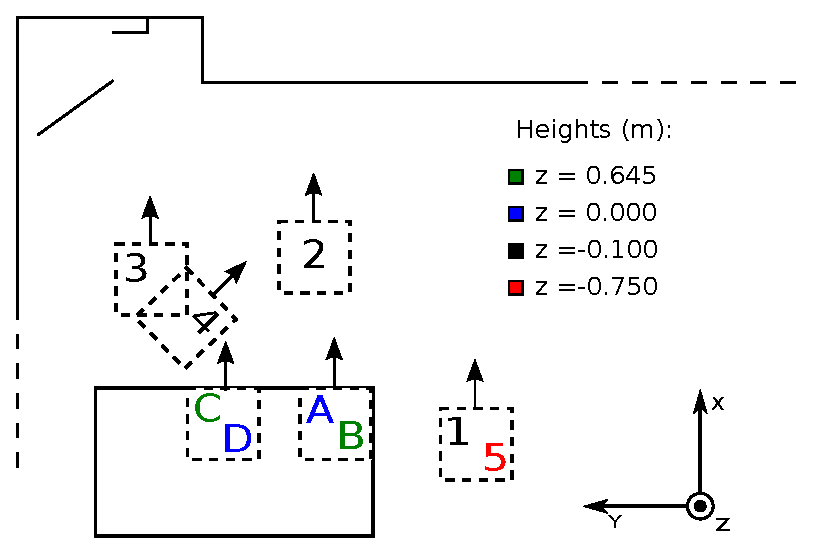
\includegraphics{benchmark_setup.eps}
  \label{fig:benchmarksetup}
  \caption{Different positions of the drone during the validation}
\end{figure}

\subsection{Experimental setup}
We will conduct two different finds of experiments: one to measure the accuracy, and one to measure the robustness of the mapping method. In both cases, we begin by placing the drone at the corner of a desk (position A on figure \ref{fig:benchmarksetup}). After the drone has saved its view, it is placed on a stool exactly above its first position. Its exact pose is then manually communicated to the drone to simulate the measurements from its IMU and ultrasonic sensor. The drone then again takes a snapshot of its camera input, and matches points with the first view, and then adjusts its second pose and the position of the points through bundle adjustment. The drone and stool are then moved to the left (position B on fiugre \ref{fig:benchmarksetup}), and again manually given its exact position, after which it takes another snapshot, matches points with the first two views, and readjusts the poses of the keyframes anf the positions of the points through bundle adjustment. This entire process is rpeated a third time when the drone is placed on the desk again at position D. The initialization of the map consists in making these four keyframes and adjusting their position and that of the landmarks 3 times. After this initialization is done, we place the drone at different locations, and measure how close it is to where it thinks it is. We evaluate the initialization based on how accurate its position estimation is, as well as on how much time the successive bundle adjustments took.


\section{Triangulation}
In the problem of triangulation, we try to find the 3D coordinates of a point from the 2D coordinates of the projection of this point on two images that were seen from different positions. We assume that the position of the camera taking these images is known exactly at both locations. If the camera positions is known exactly, and if the projection of the points into the image planes was perfect, then the two rays going from the camera centers, and through the images of the points would intersect at the location of the 3D point. In practice however, these two rays never cross exactly, so a method has to be found to find the best possible location of a 3D point from the pair of images.

\subsection{Midpoint Method}
The simplest solution would be to take the midpoint of the common perpendicular of the two rays. This method is intuitive to understand geometrically, and is quite easy to compute. In practice, however its results are not very good, as there is no theoretical reason for this point to be the best. The optiaml solution would be to displace the pixels on both images until the resulting rays meet, keeping the displacement of the pixels as small as possible (in the least squared sense). Such a solution would give the maximum likelihood estimator of the position of the 3D points, under the assumption that the error of their projection on the image planes follows gaussian noise.

\subsection{Optimal Correction}
There are several algorithms in the litterature that triangulate the position of a point using optimal correction. The most popular one, proposed by Hartley and Sturm \cite{hartleysturm}, computes the solution directly but requires finding the root of a 6th degree polynomial. Kanantani et. al.'s method \cite{kanatani} finds a solution iteratively, but requires very few iterations to have an accurate solution, and in practice, is faster than the Hartley Strum method. It also has better numerical properties, as unlike the Hartley-Sturm method, it does not have singularities at the epipoles.

\subsection{Comparison of triangulation methods}
Using the evaluation procedure described in section \ref{evalproc}, we can compare these 2 triangulation methods.

\begin{table}[H]
  \centering
  \caption{Comparison between triangulation methods}
  \small\addtolength{\tabcolsep}{-2pt}
  \begin{tabular}{ @{} l S[table-format=2.3] S[table-format=2.3] S[table-format=2.3] S[table-format=2.3] S[table-format=2.3] @{}  }
    \toprule
    {}                 & \multicolumn{2}{c}{Precision} &  \multicolumn{2}{c}{Robustness} & Computation  \\
    {}                 & {\footnotesize Distance (\si{\meter})} & {\footnotesize Angle (\si{\radian})}
    & {\footnotesize Distance (\si{\meter})} & {\footnotesize Angle (\si{\radian})} & time (\si{\second}) \\ \midrule
    Midpoint Method    & 0.114        & 0.049          &  0.827        &  0.262          &  0.012  \\
    Optimal Correction & 0.097        & 0.039          &  0.773        &  0.213          &  0.024  \\
    \bottomrule
  \end{tabular}
  \label{fig:triangcompare}
\end{table}
The computations were timed during the precision test, but these timings should be the same for the robustness tests. %TODO justify this
We can see that the optimal correction method is more performant, at the cost of being computationally heavier. We will see, however, that this computation time is negligible in comparison with the time taken for bundle adjustment. Therefore, we will use the optimal correction method to triangulate points.

\section{Bundle Adjustment}
Unfortunately the main source of errors when mapping points is not inaccuracy of the camera, but uncertainty on the camera's position. This is bad, as a bad estimation of the camera's position will result in badly located landmarks, which in turn will result in a bad estimation of the camera position. In the long term, errors will accumulate, and the map will be completely distorted. Luckily, if we have enough point correspondences between two images, it is possible to deduce the relative displacement between the two images. This means that from a set of images, we can reconstruct a scene, without even needing a prior estimation of the position of the cameras that took the images. This is good news as it means that the images can give us some absolute information about the scene, not only relative to the drone. The problem of adjusting camera positions and 3D point locations in order to minimize the reprojection errors of the 3D points onto the image planes is known as bundle adjustment. As stated above, bundle adjustment has the advantage of being absolute with respect to the world, and so not having errors accumulate. Another advantage of bundle adjustment, is that it can easily take into account points that are seen by more than two cameras, which is not trivial for the triangulation techniqhes described above. The main disadvantage of bundle adjustment is that it is computationally heavy, so it is important to adapt it to be useable un real time.\\
To show the advantages of bundle adjustment, we compare it with triangulation using the optimal correction method. When using bundle adjustment, optimal correction triangulation is also used to obtain an initial solution, from which we optimize.
\begin{table}[H]
  \centering
  \caption{Performance of Bundle Adjustment}
  \small\addtolength{\tabcolsep}{-2pt}
  \begin{tabular}{ @{} l S[table-format=2.3] S[table-format=2.3] S[table-format=2.3] S[table-format=2.3] S[table-format=2.3] @{}  }    \toprule
    {}      & \multicolumn{2}{c}{Precision} &  \multicolumn{2}{c}{Robustness} & Computation time (\si{\second}) \\
    {}      & {\footnotesize Distance (\si{\meter})} & {\footnotesize Angle (\si{\radian})}
    & {\footnotesize Distance (\si{\meter})} & {\footnotesize Angle (\si{\radian})} & time (\si{\second}) \\ \midrule
    No Bundle Adjustment   & 0.097        & 0.039          &  0.773        &  0.213          &  0.024  \\
    With Bundle Adjustment & 0.091        & 0.031          &  0.592        &  0.221          &  13.232\\
    \bottomrule
  \end{tabular}
  \label{fig:bacompare}
\end{table}
We see that bundle adjustment gives a significant improvement to the performance of the pose estimation. However, we see that the errors in the case of the robustness test are still quite high, with an average position error of \SI{59.2}{\centi\meter}, and an average orientation error of \SI{0.221}{\radian}. More importantly, the total time taken for bundle adjustment was a bit over \SI{13}{\second}, which is a prohibitively large amount of time for real time applications. The following parts of this section will be focused on reducing this time, and increasing the robustness of the mapping (measured by the performance under noisy pose estimation).

\subsection{Convergence of the solver}
The first element we can tune is the convergence criterion of the solver that solves the bundle adjustment problem. We will stop either when the ration of the change in the objective function to the value of this function arrives below some threshold. This ensures that the criterion scales with the problem, which is important as the size of the problem can vary during operation (as the map grows, for example). The default value of the Ceres solver is $10^{-6}$, but experimentally, we find that use a less severe threshold, to significantly speed up the computations, without impactig the quality of the results too much.
\begin{table}[H]
  \centering
  \caption{Effect of convergence criterion on Bundle Adjustment speed and performance}
  \small\addtolength{\tabcolsep}{-2pt}
  \begin{tabular}{ @{} l S[table-format=2.3] S[table-format=2.3] S[table-format=2.3] @{}  }    \toprule
    {Convergene Threshold}  & { Distance (\si{\meter})} & { Angle (\si{\radian})} & {Time (\si{\second})}     \\ \midrule
    10                      &     0.0975  &   0.0378  &     0.536  \\
    5                       &     0.0967  &   0.0397  &     0.530  \\
    1                       &     0.0989  &   0.0406  &     0.521  \\
    0.5                     &     0.0970  &   0.0393  &     0.520  \\
    0.1                     &     0.1065  &   0.0431  &     0.646  \\
    0.05                    &     0.1385  &   0.0462  &     0.761  \\
    0.04                    &     0.1380  &   0.0454  &     0.754  \\
    0.03                    &     0.1575  &   0.0531  &     1.130  \\
    0.02                    &     0.0793  &   0.0255  &     1.354  \\
    0.01                    &     0.0722  &   0.0278  &     1.425  \\
    0.005                   &     0.0765  &   0.0257  &     1.544  \\
    0.001                   &     0.0879  &   0.0271  &     3.595  \\
    0.0001                  &     0.0978  &   0.0330  &     5.207  \\
    0.00001                 &     0.0916  &   0.0317  &     12.620 \\
    0.000001                &     0.0789  &   0.0307  &     13.232 \\
    0.0000001               &     0.0816  &   0.0229  &     15.453 \\
    \bottomrule
  \end{tabular}
  \label{fig:convergencetol}
\end{table}



\section{Tuning the Bundle Adjustment}
The main drawback of Bundle Adjustment is that it requires an iterative method to be solved and can take a lot of time, which of course is a limiting factor for a robot that builds a map in real time. Therefore it is important to optimize both the speed of the computations, and their precision. As is often the case, there will have to be a tradeoff between these two. To measure both the speed of the Bundle Adjustment and the accuracy of the map obtained, we will conduct some experiments using different parameters to initialize the map.





\section{Map Initialization}
A robot needs a map lo localize itself within it, but it needs to know its position to find the postion of surrounding objects and build a map. Because the mapping and localization tasks are mutually dependent on one another, there needs to be a special procedure to build a map from nothing when it does not exist yet. Arbitrarily, we decide that the position of the drone when it starts flying is the origin (in all 6 degrees of freedom) of the map. However, with only a monocular camera, it is not possible to find the exact location of any visual features from one observation only, views from at least two different positions are needed to triangulate points.


%%blabla

To reach the position from which the drone will take a second view and triangulate points, the drone has to fly blindly. Blindly here means without using a map la localize itself visually, but the drone can still use its other sensors (IMU and ultrasonic sensor) to obtain an estimate of its postion. Because the ultrasonic sensor is much more accurate than the IMU, and gives an absolute measure, we will mostly rely on this sensor to estimate the relative position from where we take the second view. Because the ultrasonic sensor only gives the distance from the bottom of the drone to the ground, the drone should fly straight up from its first position (the origin) to reach its second position.\\
Once in its second position, the drone can match seen keypoints from both views, and from its estimated position, triangulate those points to the map. However, the drone's estimation of its pose is prone to errors, especially as it only used its ultrasonic sensor and IMU. There errors can be corrected with the information from the cameras, because of we have %TODO how many
matching observations, we can compute the fundamental matrix, and know exactly the displacement between the two views. Refining the poses of the views and the location of the landmarks simultaneously such as to minimize the reprojection error is a nonlinear optimization problem known as Bundle Adjustment. Using Bundle adjustment, we can refine the position of the second view, and use the ultrasonic sensor information to fix the scale. Another advantage of Bundle Adjustment is that it allows to take into account more than 2 views of a point.
